\documentclass[aspectratio=169]{beamer}

% Pacotes essenciais
\usepackage[utf8]{inputenc}
\usepackage[T1]{fontenc}
\usepackage[brazilian]{babel}
\usepackage{graphicx}
\usepackage{tikz}

% Fonte moderna Roboto
\usepackage[sfdefault]{roboto}
\usepackage[T1]{fontenc}

% Definição das cores
\definecolor{vermelhoPrincipal}{HTML}{b11116}
\definecolor{azulComplementar}{HTML}{3a5461}
\definecolor{brancoFundo}{HTML}{FFFFFF}

% Configuração do tema
\usetheme{Madrid}
\usecolortheme{default}

% Cores personalizadas - texto sempre em preto
\setbeamercolor{structure}{fg=black}
\setbeamercolor{palette primary}{bg=vermelhoPrincipal,fg=white}
\setbeamercolor{palette secondary}{bg=azulComplementar,fg=white}
\setbeamercolor{palette tertiary}{bg=vermelhoPrincipal,fg=white}
\setbeamercolor{palette quaternary}{bg=azulComplementar,fg=white}
\setbeamercolor{frametitle}{bg=vermelhoPrincipal,fg=white}
\setbeamercolor{background canvas}{bg=brancoFundo}
\setbeamercolor{title}{fg=black}
\setbeamercolor{subtitle}{fg=azulComplementar}
\setbeamercolor{author}{fg=black}
\setbeamercolor{date}{fg=black}
\setbeamercolor{itemize item}{fg=black}
\setbeamercolor{itemize subitem}{fg=black}
\setbeamercolor{enumerate item}{fg=black}
\setbeamercolor{block title}{bg=vermelhoPrincipal,fg=white}
\setbeamercolor{block body}{bg=vermelhoPrincipal!10,fg=black}
\setbeamercolor{normal text}{fg=black}

% Configurar fonte dos itemize
\setbeamerfont{itemize/enumerate body}{size=\scriptsize}
\setbeamerfont{itemize/enumerate subbody}{size=\scriptsize}

% Marcadores modernos e minimalistas
\setbeamertemplate{itemize item}{\raisebox{0.2ex}{\rule{0.6ex}{0.6ex}}}
\setbeamertemplate{itemize subitem}{\raisebox{0.3ex}{\rule{0.4ex}{0.4ex}}}
\setbeamertemplate{itemize subsubitem}{\raisebox{0.35ex}{\rule{0.3ex}{0.3ex}}}
\setbeamertemplate{enumerate items}[square]

% Transições suaves
\setbeamercovered{transparent}

% Remover símbolos de navegação
\setbeamertemplate{navigation symbols}{}

% Customizar o cabeçalho com barra vermelha e logo
\setbeamertemplate{headline}{
  \begin{beamercolorbox}[wd=\paperwidth,ht=0.6cm,dp=0.15cm,leftskip=0.2cm,rightskip=0.4cm]{palette primary}
    \raisebox{-0.05cm}{
\includegraphics[height=0.45cm]{imgs/base/fatec-rgt.png}}
    \hfill
    \raisebox{-0.18cm}{
\includegraphics[height=0.85cm]{imgs/base/governo-sp-secretaria-logo.png}}
    \hspace{0.2cm}
    \raisebox{-0.08cm}{
\includegraphics[height=0.6cm]{imgs/base/cps-logo.png}}
  \end{beamercolorbox}
}
% Remover sombras dos blocks
\setbeamertemplate{blocks}[default]
\setbeamertemplate{itemize/enumerate body begin}{\scriptsize}
\setbeamertemplate{itemize/enumerate subbody begin}{\scriptsize}
% Customizar o rodapé
\setbeamertemplate{footline}{
  \begin{beamercolorbox}[wd=\paperwidth,ht=0.4cm,dp=0.2cm,leftskip=0.3cm,rightskip=0.3cm]{palette secondary}
    \usebeamerfont{footline}
    \insertshortauthor \hfill \hfill {\fontsize{5}{6}\selectfont\insertshorttitle} \hfill \hfill \insertframenumber/\inserttotalframenumber
  \end{beamercolorbox}
}

% Customizar título do frame
\setbeamertemplate{frametitle}{
  \vspace{0.3cm}
  \textcolor{black}{\insertframetitle}
  \vspace{0.1cm}
}

% Informações da apresentação
\title{Teste de Desempenho Contínuo, \\ Orientado Por Rastreamento Ocular}
\subtitle{}
\author[DSM]{COSTA, A.; FUDALI, A.; CLAUDIO, D.; SANTOS, G.; GOMES, I.}
\institute{Desenvolvimento de Software Multiplataforma\\FATEC Registro}
\date{\today}

\begin{document}

% Slide de título moderno
\begin{frame}
  \vspace{0.8cm}
  \begin{center}
    \begin{tikzpicture}
      % Linha decorativa superior
      \draw[vermelhoPrincipal, line width=2pt] (-4,0) -- (4,0);
    \end{tikzpicture}
    
    \vspace{0.4cm}
    
    {\normalsize\bfseries\inserttitle}\par
    
    \vspace{0.2cm}
    
    {\tiny\insertauthor}\par
    
    \vspace{0.1cm}
    
    {\small\textcolor{azulComplementar}{\insertsubtitle}}\par
    
    \vspace{0.5cm}
    
    \begin{tikzpicture}
      % Linha decorativa inferior
      \draw[azulComplementar, line width=1.5pt] (-2.5,0) -- (2.5,0);
    \end{tikzpicture}
    
    \vspace{0.3cm}
    
    {\scriptsize\insertinstitute}\par
    
    \vspace{0.01cm}
    
    {\tiny\textcolor{azulComplementar}{\insertdate}}\par
  \end{center}
\end{frame}

\section{Agenda}
{
% Slide de agenda
\usebackgroundtemplate{%
  
\includegraphics[width=\paperwidth,height=\paperheight]{imgs/agenda.png}%
}
\begin{frame}[b]{Agenda}
  \begin{itemize}
    \item Pitch
    \item Problematização
    \item Estado da Arte
    \item Objetivo
    \item Ferramental
    \item Metodologia
    \item Apresentação prática
    \item Resultados e Discussões
  \end{itemize}
  
  \vfill
  
  {\scriptsize \textbf{Duração:} 10 a 11 min.}
\end{frame}
}

\section{Pitch}
{
\usebackgroundtemplate{%
  
\includegraphics[width=\paperwidth,height=\paperheight]{imgs/pitch.jpg}%
}
\begin{frame}[b]{\textcolor{white}{Pitch}}

\end{frame}
}

\section{Problematização}

{
\usebackgroundtemplate{%
  
\includegraphics[width=\paperwidth,height=\paperheight]{imgs/problematizacao.png}%
}
\begin{frame}[b]{Problematização}
  \begin{itemize}
   \item Diagnóstico tradicional de TDAH é subjetivo e inacessível.
  \item Falta de ferramentas tecnológicas acessíveis.
  \item Necessidade de métricas como movimento ocular para fundamentar \\ a análise clínica.
  \item Baixo engajamento em processos avaliativos tradicionais.
  \end{itemize}
  
  \vfill
  
  {\fontsize{4}{5}\selectfont\textit{Fonte: Blog Rede Sagrado}\hfill\textcolor{white}{Imagem: Aluna pensativa}}
\end{frame}
}

\section{Objetivo}

{
\usebackgroundtemplate{%
  
\includegraphics[width=\paperwidth,height=\paperheight]{imgs/objetivos.png}%
}
\begin{frame}[b]{Objetivo}
  \begin{itemize}
    \item \parbox{0.60\textwidth}{\textbf{Objetivo geral}: Desenvolver uma plataforma digital gamificada para triagem inicial de TDAH em crianças de 10 a 12 anos, utilizando tecnologias acessíveis.}
    \item \parbox{0.60\textwidth}{\textbf{Objetivos específicos}:}
    \begin{itemize}
      \item \parbox{0.55\textwidth}{Integrar o TDC ao ambiente lúdico}
      \item \parbox{0.55\textwidth}{Aplicar Eye Tracking em tempo real}
      \item \parbox{0.55\textwidth}{Processar dados via IA}
      \item \parbox{0.55\textwidth}{Fornecer relatório clínico intuitivo}
    \end{itemize}
  \end{itemize}
  
  \vfill
  
  {\fontsize{4}{5}\selectfont\textit{Fonte: Fonte própria}\hfill\textcolor{white}{Imagem: Fase 1 - FocusQuest}}
\end{frame}
}

\section{Estado da Arte}

\begin{frame}[t]{Estado da Arte}
  \scriptsize  
  \begin{table}
    \centering
    \tiny
    \begin{tabular}{|p{2.5cm}|p{2cm}|p{2cm}|p{2cm}|p{2cm}|p{1.5cm}|}
      \hline
      \textbf{Título/Autores} & \textbf{Objetivo} & \textbf{Método} & \textbf{Resultados} & \textbf{Limitações} & \textbf{Gap} \\
      \hline
      Attention-Deficit/Hyperactivity Disorder (ADHD): Integrating the MOXO-dCPT with an Eye Tracker Enhances Diagnostic Precision — Elbaum et al. (2020) & Avaliar os níveis de distratibilidade atencional em pacientes com TDAH & Uso do teste MOXO-dCPT combinado com rastreamento ocular comercial (Eye Tracking) & Demonstrou alta precisão discriminativa na identificação de padrões visuais de desatenção & Alto custo financeiro, exigência de hardware proprietário e necessidade de aplicação em ambiente clínico controlado & Inacessibilidade financeira e falta de validação para o público infantil (10-12 anos) \\
      \hline
      Virtual reality-assisted prediction of adult ADHD based on eye tracking, EEG, actigraphy and behavioral indices: a machine learning analysis of independent training and test samples — Wiebe et al. (2024) & Propor um ambiente de diagnóstico imersivo para transtornos de atenção & Realidade Virtual (VR) + Eletroencefalograma (EEG) + Eye Tracking com suporte de Inteligência Artificial & Alcançou 81\% de acurácia na classificação de TDAH utilizando modelos preditivos & Equipamentos altamente intrusivos para crianças (óculos VR e sensores EEG) e zero escalabilidade para saúde pública & Zero escalabilidade para triagem rápida em ambientes não clínicos ou remotos \\
      \hline
      A RELAÇÃO ENTRE A PRÁTICA REGULAR DE VIDEOGAMES E ATENÇÃO SUSTENTADA — Nascimento e Menezes (2020) &Explorar relação entre videogames e atenção sustentada & Uso do teste CPT II em jogadores e não jogadores & Diferenças apenas por sexo; sem impacto direto do gênero do jogo & Necessidade de maior controle metodológico e de variáveis & Falta de um marcador fisiológico objetivo e foco em diagnóstico clínico \\
      \hline
    \end{tabular}
  \end{table}
\end{frame}

\section{Ferramental}

{
\usebackgroundtemplate{%
  
\includegraphics[width=\paperwidth,height=\paperheight]{imgs/ferramentas.png}%
}
\begin{frame}[b]{Ferramental}
  \begin{itemize}
    \item \parbox{0.60\textwidth}{\textbf{Linguagens}: JavaScript, TypeScript e Python}
    \item \parbox{0.60\textwidth}{\textbf{Frameworks}: React, Next.js, Node.js e Express}
    \item \parbox{0.60\textwidth}{\textbf{Bibliotecas}: WebGazer, Scikit-learn, Pandas e Uvicorn}
    \item \parbox{0.60\textwidth}{\textbf{Banco de dados e persistência}: MongoDB e Redis}
    \item \parbox{0.60\textwidth}{\textbf{Infraestrutura}: GCP, Docker e Mongo Atlas}
    \item \parbox{0.60\textwidth}{\textbf{Ferramentas}: Git, VS Code, Figma e Swagger}
  \end{itemize}
  
  \vfill
  
  {\fontsize{4}{5}\selectfont\textit{Fonte: Freepik}\hfill\textcolor{white}{Imagem: Astronauta com um notebook}}
\end{frame}
}

\section{Metodologia}

{
\begin{frame}[t]{Metodologia}
  
  \vspace{-0.5cm} 
  
  \begin{center}
    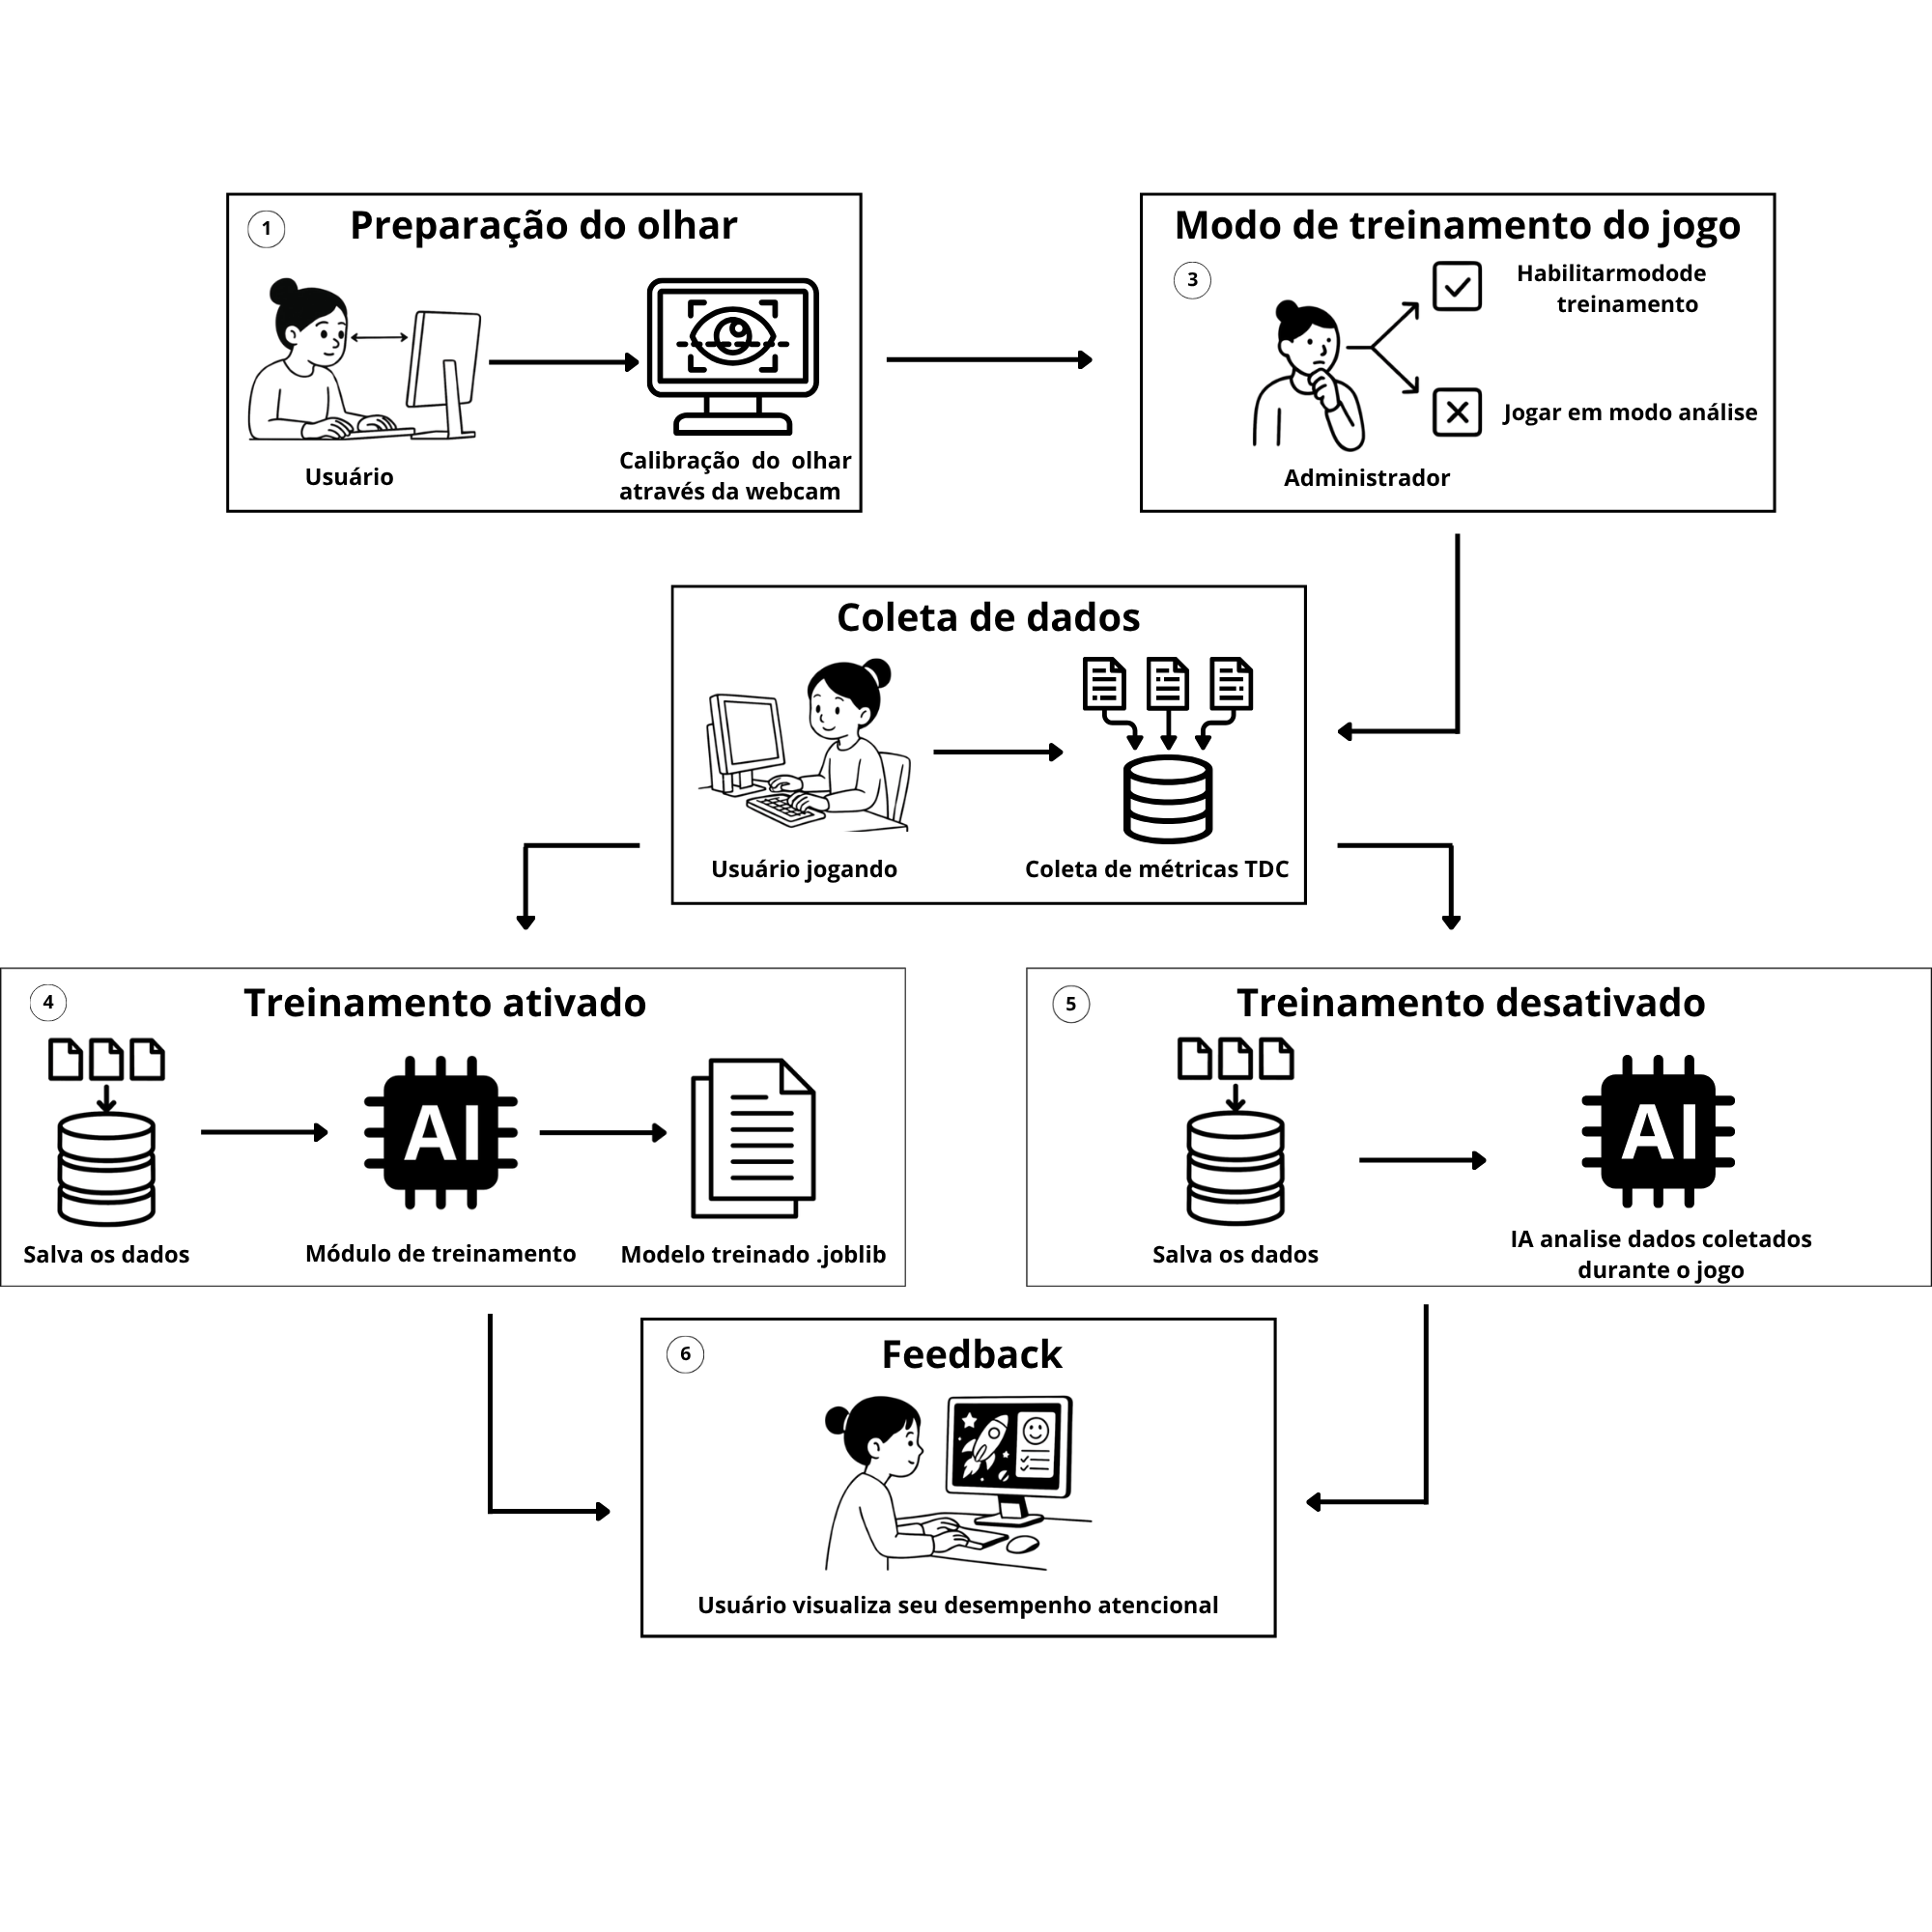
\includegraphics[width=\textwidth,height=1\textheight,keepaspectratio]{imgs/metodologia.png}
  \end{center}

\end{frame}
}

\section{Apresentação Prática}

{
\usebackgroundtemplate{%
  
\includegraphics[width=\paperwidth,height=\paperheight]{imgs/apresentacao.png}%
}
\begin{frame}[b]{Apresentação Prática}
  \begin{itemize}
    \item \parbox{0.60\textwidth}{Demonstração das 3 fases do jogo com eye tracking em tempo real}
    \item \parbox{0.60\textwidth}{Exibição de métricas coletadas e comparação \\ com parâmetros de referência}
    \item \parbox{0.60\textwidth}{Geração de feedback imediato e relatório clínico simplificado}
    \item \parbox{0.60\textwidth}{Integração da IA no projeto}
  \end{itemize}
  
  \vfill
  
  {\fontsize{4}{5}\selectfont\textit{Fonte: Freepik}\hfill\textcolor{white}{Imagem: Astronauta mexendo no notebook}}
\end{frame}
}

\section{Resultados e Discussões}

{
\begin{frame}[t]{Resultados e Discussões}
  \small

  \begin{block}{Resultados}
    \textbullet~ Validação inicial do protótipo \newline
    \textbullet~ Sucesso na integração do IoT (Arduino) \newline
    \textbullet~ Sucesso no registro de métricas e geração de relatórios\newline
    \textbullet~ Implementação de IA para análise preditiva
  \end{block}

  \begin{columns}[t]
    \begin{column}{0.48\textwidth}
      \begin{block}{Dificuldades}
        \textbullet~ Precisão do \textit{eye tracking} em diferentes ambientes \newline
        \textbullet~ Necessidade de dados reais para a IA
      \end{block}
    \end{column}
    
    \begin{column}{0.48\textwidth}
      \begin{block}{Próximos Passos}
        \textbullet~ Coleta de dados com participantes reais e validação clínica
      \end{block}
    \end{column}
  \end{columns}

  \vspace{0.2cm}
  \scriptsize
  Os resultados indicam viabilidade técnica e potencial de democratização do diagnóstico, mas ainda são necessários avanços em validação clínica, escalabilidade e precisão dos dados.
\end{frame}
}

% Slide Informações Gerais (clone)
{
\usebackgroundtemplate{%
  
\includegraphics[width=\paperwidth,height=\paperheight]{imgs/fim.png}%
}
\begin{frame}[b]{}
  \vspace{0.2cm}
  
  \hspace*{0.25\paperwidth}{\Large \textbf{Obrigado!}}
  
  \vfill
\end{frame}
}

\end{document}
